\documentclass{article}

\usepackage{graphicx}
\usepackage{amsmath,amssymb}
\usepackage{mathtools}
%\usepackage{etoolbox}
%\usepackage{booktabs}
\usepackage{float}
\usepackage{geometry}
%\usepackage{multicol}
%\usepackage{caption}
\usepackage[outdir=./eps2pdf/]{epstopdf}
\graphicspath{
  {figures/}
  {figures/goals/}
  {figures/light_data/}
  {figures/attenuation/}
}

\begin{document}
\section{RTE: 1D}

\section{RTE: Vector}

\section{Asymptotics}

\section{Physical Interpretation}

\section{Numerical Implementation}
\subsection{Grid}

\begin{figure}
  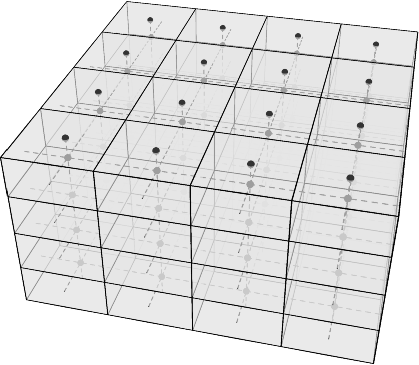
\includegraphics[width=8cm]{spatialgrid}
  \caption{Spatial grid}
\end{figure}

\begin{figure}
  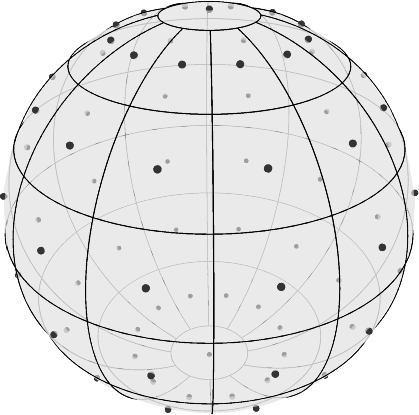
\includegraphics[width=8cm]{angulargrid}
  \caption{Angular grid}
\end{figure}



\end{document}